\chapter{Firewall}
Die Firewall wird in dem Praktikum mit IPTables von Linux realisiert. Dies ermöglicht das Aufstellen von Regeln, welche in Tabellen abgelegt werden, um Verbindungen zwischen zwei Netzen zu kontrollieren. Wenn ein Paket die Firewall erreicht, dann checkt die Firewall sequentiell die einzelnen Regeln und wenn eine Zutrifft wird der zugehörige ACCEPT oder DROP auf das Paket angewandt. Bei ACCEPT wird das Paket weiter gereicht und bei DROP wird das Paket einfach fallen gelassen und der Zielrechner erhält nicht das Paket. Wenn keine Regel zutrifft, dann wird die Default Policy angewandt. Diese kann wiederum auf DROP und ACCEPT gesetzt sein. 
\begin{figure}
	\centering
		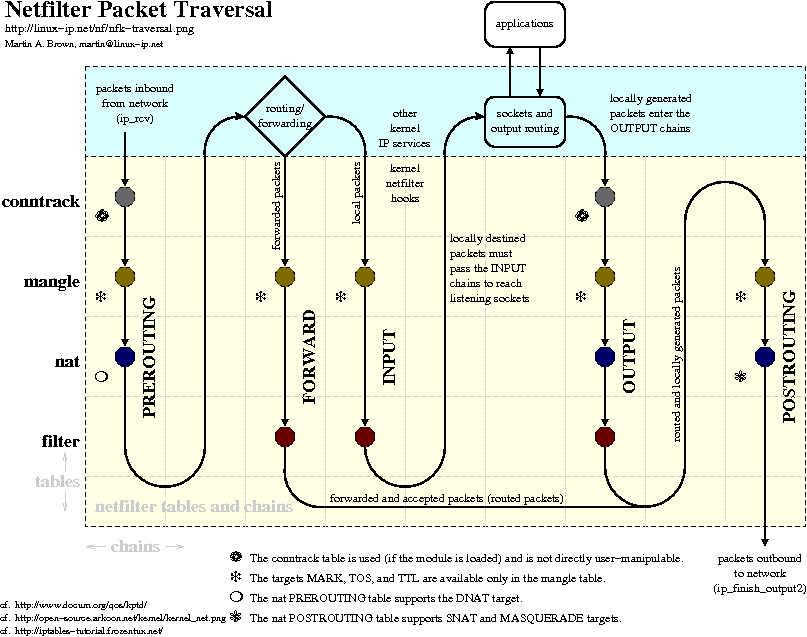
\includegraphics[width=1.00\textwidth]{figures/firewall_uebersicht.PNG}
	\caption{Firewall Übersicht \cite{linux-ip}}
	\label{fig:firewall_uebersicht}
\end{figure}
In der Abbildung \ref{fig:firewall_uebersicht} ist zu sehen das es verschiedene Tabellen gibt. Je nachdem ob des Paket weitergeleitet wird oder einen lokalen Prozess als Ziel hat, werden die zuständigen Tabellen geprüft. Folgend eine kurze Erklärung, wann welche Tabelle genutzt wird.
\begin{itemize}
	\item PREROUTING \\
	Hier landen Pakete bevor entschieden worden ist, ob das Paket weitergeleitet wird oder einen lokalen Prozess als Ziel hat.
	\item POSTROUTING \\
	Ganz zum schluss, wenn schon alle vorherigen Entscheidungen getroffen worden sind wird laufen die Pakete hier nochmals durch.
	\item FORWARD \\
	Hierbei handelt es sich um ein Paket, welches weitergeleitet wird.
	\item INPUT \\
	Das Paket hat einen lokalen Prozess, auf dem Rechner wo die Firewall läuft, als Ziel.
	\item OUTPUT \\
	Hierbei handelt es sich um ein Paket, welche von einem lokalen Prozess abgesendet wird.
\end{itemize}
Die Regeln beschränken sich auf die Schicht 3 und 4 von den zu übertragenden Paketen. Somit hat man Zugriff auf die Übertragungsflags, IP-Adressen, Ports und die zugehörigen Netzwerkinterfaces. IPTables ermöglicht verbindungsorientierte Paketfilter, somit kann zum Beispiel überprüft werden ob eine Verbindung related ist, dass heißt es wird eine Unterverbindung aufgebaut, wo schon eine Verbindung zwischen den Rechnern besteht. Des weiteren ermöglicht IPTables eine NAT mit Masquerade Funktion. Das bedeutet es versteckt die Rechner von einem Netzwerk vor dem anderen.

\

 Damit die Regeln nach einem Neustart des Rechners erhalten werden. Müssen diese in eine Datei ausgelagert werden.


\section{Anforderungen}
Indem Praktikumsaufbau gibt es zwei Firewalls. Hierbei handelt es sich um eine Äußere Firewall, welche wie in Abbildung \ref{fig:Netzplan} zu erkennen die Verbindungen zwischen der DMZ und dem Internet regelt. Und die Rechner aus der DMZ werden vor Rechnern aus dem Internet versteckt. Die innere Firewall hat dabei dieselben Aufgaben nur ist sie zwischen der DMZ und dem Firmennetzwerk platziert.

\subsection{Innere Firewall}
\begin{itemize}
\item Masquerading von dem Firmennetz zur DMZ. Somit dürfen die IP Adressen der Rechner aus dem Firmennetz in der DMZ nicht erkennbar sein, sondern als IP Adresse ist die der Firewall zu sehen.
\item Es dürfen keine neuen Verbindungen von der DMZ in das interne Firmennetz aufgebaut werden.
\item Rechner aus dem Firmen internen Netzwerk dürfen neue Verbindungen zur DMZ und dem Internet aufbauen.
\item Auf der inneren Firewall läuft der VPN Prozess und dieser muss aus dem Internet erreichbar sein.	
\end{itemize}

\subsection{Äußere Firewall}
\begin{itemize}
\item Masquerading von der DMZ zum Internet.
\item Der Webserver aus der DMZ soll von dem Internet über die üblichen Ports erreichbar sein. Darunter fallen folgende Ports. 80(HTTP), 443(HTTPS), 25(SMTP), 587(SMTP), 465(SMTPS), 993(IMAPS), 995(POP3S), 143(IMAP), 110(POP3), 53(DNS)
\item Die interne Firewall muss erreichbar sein für das VPN. Somit müssen folgende Ports auf die innere Firewall weitergeleitet werden. 1195(VPN: Client to Lan), 1194(VPN: Lan to Lan)
\end{itemize}




